\documentclass{zjureport}
% =============================================
% Part 0 Edit the info
% =============================================

\major{计算机体系结构}
\name{卞留念}
\title{实验报告}
\stuida{201828013229131}
\stuidb{2018E8013261055}
\college{计算机学院}
\date{\zhtoday}
\lab{寝室}
\course{计算机网络}
\instructor{谢高岗}
\expname{静态路由转发实验}
\exptype{设计实验}
\partner{卫一宁}

\begin{document}
% =============================================
% Part 1 Header
% =============================================
\makecover
\makeheader

% =============================================
% Part 2 Main document
% =============================================

\section{实验要求}
  本实验要求学生在已有代码基础上,完善其中的TODO部分,实现路由器的IP查找转发、ARP请求和应答、ARP缓存管理、发送ICMP消息等功能。
\section{实验内容和步骤}

  \subsection{实验内容一}

      \begin{enumerate}
          \item 运行给定网络拓扑(router\_topo.py)
          \item Ping 10.0.1.1 (r1),能够ping通
          \item Ping 10.0.2.22 (h2),能够ping通
          \item Ping 10.0.3.33 (h3),能够ping通
          \item Ping 10.0.3.11,返回ICMP Destination Host Unreachable
          \item Ping 10.0.4.1,返回ICMP Destination Net Unreachable
      \end{enumerate}

  \subsection{实验内容二}


      \begin{enumerate}
          \item 构造一个包含多个路由器节点组成的网络,手动配置每个路由器节点的路由表,有两个终端节点,通过路由器节点相连,两节点之间的跳数不少于3跳,手动配置其默认路由表
          \item 终端节点ping每个路由器节点的入端口IP地址,能够ping通
          \item 在一个终端节点上traceroute另一节点,能够正确输出路径上每个节点(入端口)的IP信息
      \end{enumerate}

\section{主要仪器设备}
  计算机,Mininet 软件,Wireshark 软件

\section{实验步骤}
  \subsection{安装mininet与wireshark软件}
      下载并安装mininet与wireshark等软件。
  \subsection{编写代码TODO部分}
      根据所学知识完成代码的TODO部分。
  \subsection{完成实验内容}
      编译代码生成程序,在路由器节点上运行此程序,依次完成实验内容。

\section{实验过程}
  \subsection{安装mininet与wireshark软件}
     在Ubuntu下输入sudo apt install mininet 与 sudo apt install build-essential xterm wireshark ethtool iperf traceroute iptables arptables命令进行软件安装,安装完成后,运行sudo mn验证mininet是否正确安装,验证结果如图~\ref{fig:install} 所示。
           \begin{figure}[!htbp]
               \centering
               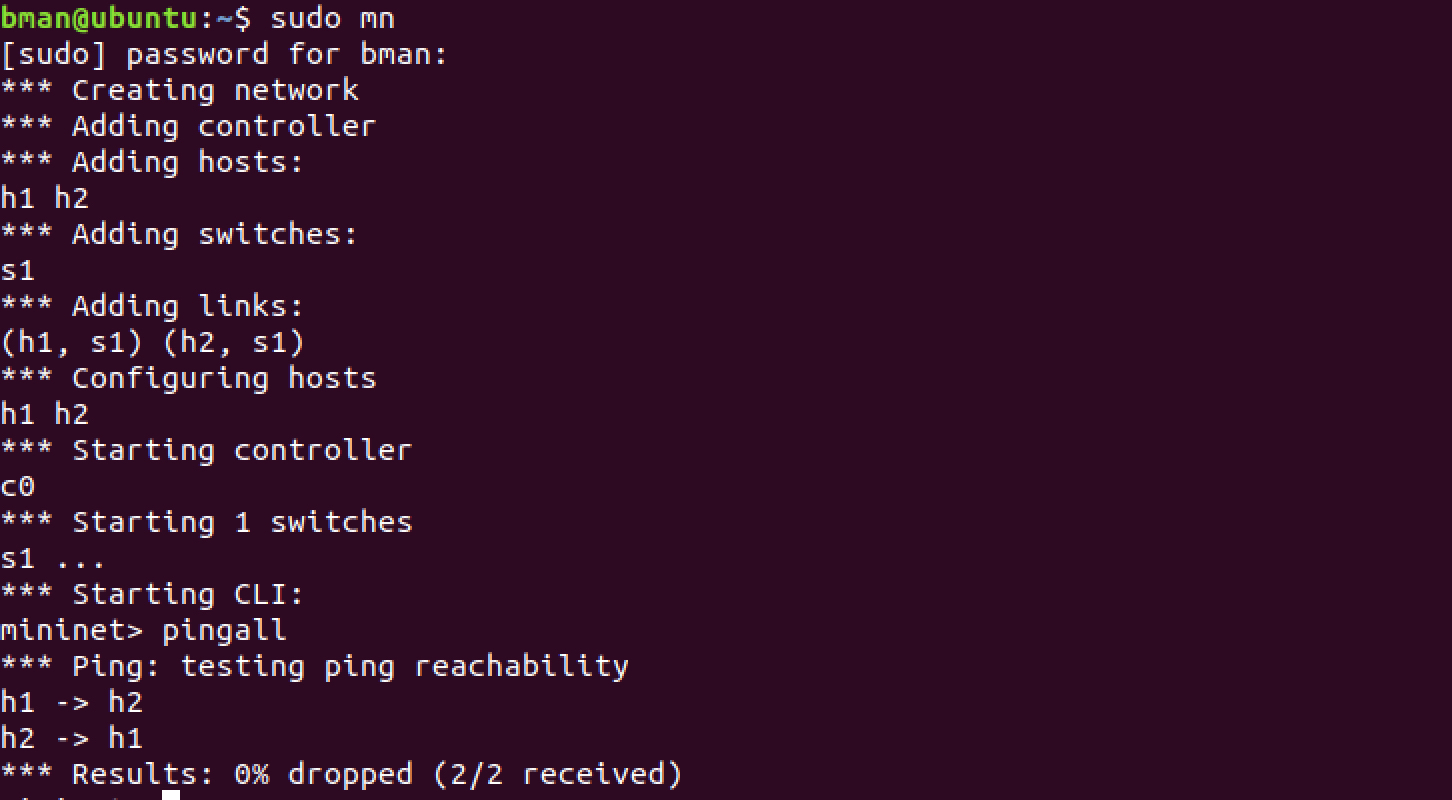
\includegraphics[width=0.7\linewidth]{figures/02.jpg}
               \caption{mininet成功安装验证图}
               \label{fig:install}
           \end{figure}

  \subsection{编写arpcache\_lookup函数}
      \lstinputlisting[language=C]{code/arpcache_lookup.c}

  \newpage
  \subsection{编写arpcache\_append\_packet函数}
      \lstinputlisting[language=C]{code/arpcache_append_packet.c}

  \newpage
  \subsection{编写arpcache\_insert函数}
    \lstinputlisting[language=C]{code/arpcache_insert.c}

  \newpage
  \subsection{编写arpcache\_sweep函数}
    \lstinputlisting[language=C]{code/arpcache_sweep.c}

  \newpage
  \subsection{编写arp\_send\_request函数}
    \lstinputlisting[language=C]{code/arp_send_request.c}

  \newpage
  \subsection{编写arp\_send\_reply函数}
    \lstinputlisting[language=C]{code/arp_send_reply.c}

  \newpage
  \subsection{编写handle\_arp\_packet函数}
    \lstinputlisting[language=C]{code/handle_arp_packet.c}

  \subsection{编写iface\_send\_packet\_by\_arp函数}
    \lstinputlisting[language=C]{code/iface_send_packet_by_arp.c}

  \newpage
  \subsection{编写longest\_prefix\_match函数}
    \lstinputlisting[language=C]{code/longest_prefix_match.c}

  \subsection{编写handle\_ip\_packet函数}
    \lstinputlisting[language=C]{code/handle_ip_packet.c}

  \newpage
  \subsection{编写icmp\_send\_packet函数}
    \lstinputlisting[language=C]{code/icmp_send_packet.c}

  \subsection{编写ip\_forward\_packet函数}
    \lstinputlisting[language=C]{code/ip_forward_packet.c}

  \newpage
  \subsection{完成实验内容一}
      \begin{enumerate}
          \item 运行router\_topo.py生成的网络结构如图~\ref{fig:rtpy} 所示。
                \begin{figure}[!htbp]
                    \centering
                    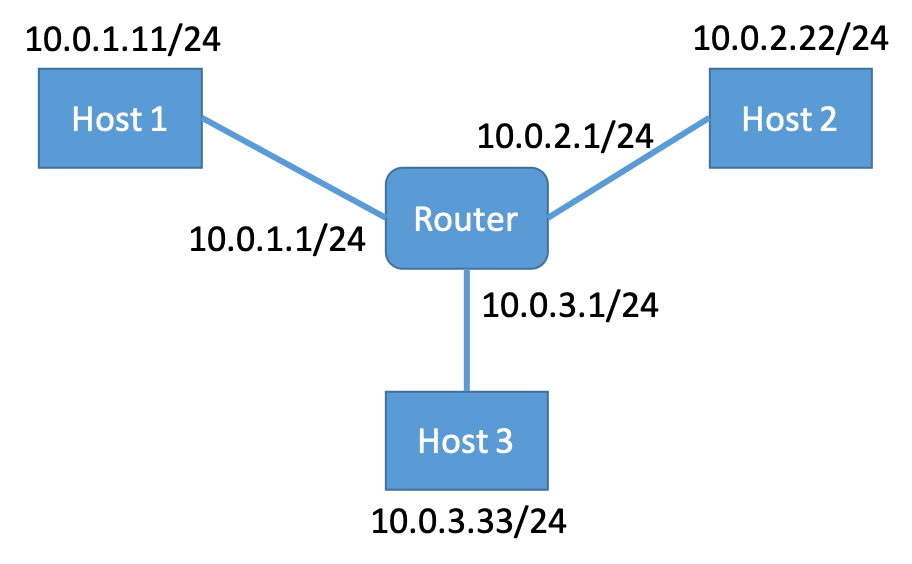
\includegraphics[width=0.7\linewidth]{figures/rtpy.png}
                    \caption{router\_topo.py生成的网络}
                    \label{fig:rtpy}
                \end{figure}

      \end{enumerate}

  \subsection{完成实验内容二}


\section{实验结果与分析}

\section{说明}


\end{document}
